\section{Testy rozwiązania}
	\label{final:testy}

	\subsection{Generowanie grafów}
		\label{final:testy:generowanie}

		Istotnym etapem projektu było przygotowywanie danych testowych. Do tego celu został zaimplementowany generator grafów(klasa GraphGenerator). Generowane grafy były zapisywane do pliku w celu ich późniejszego wykorzystania do analizy. Etap generowania grafów był etapem, który zajął najwięcej czasu w procesie testowania i wynosił on kilka dni. Grafy, które zostały wygenerowane zajęły około 10 GB pamięci na dysku.
% \\
% TABELKA
% \\
% \\
	\subsection{Testowanie}
		\label{final:testy:przyklad1}
		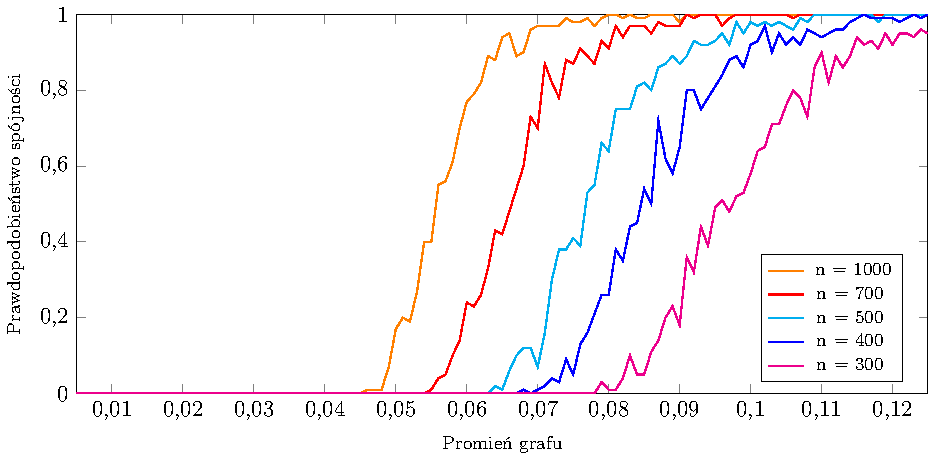
\includepdf[scale=0.9, pages={1}]{500-0_0010_125_consistency_prob.pdf}
		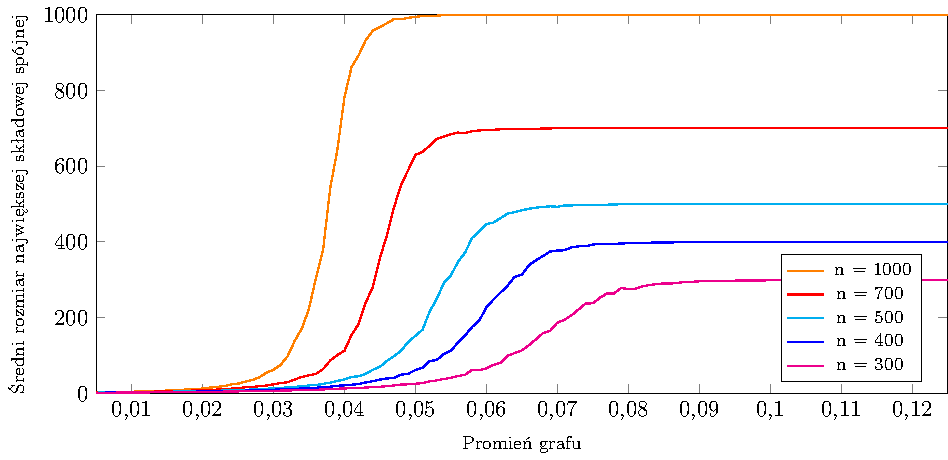
\includepdf[scale=0.9, pages={1}]{500-0_0010_125_max_comps_sizes_means.pdf}
		%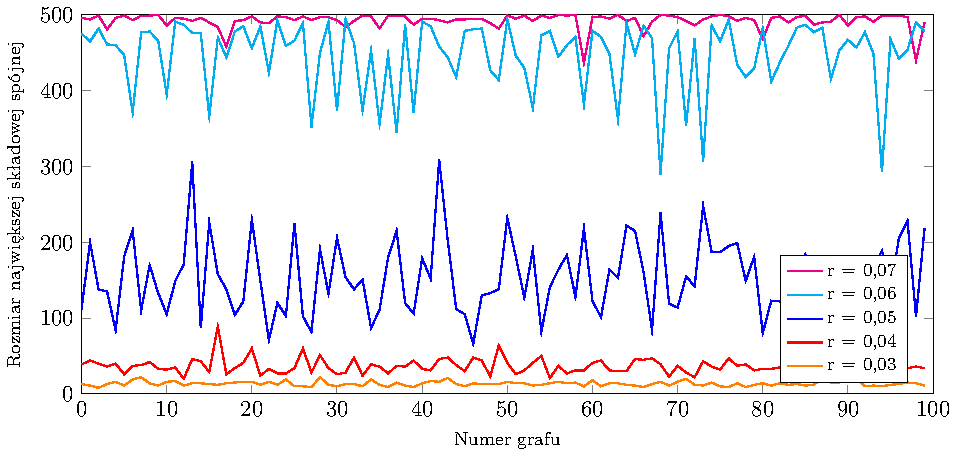
\includepdf[scale=0.8, pages={1}]{500-max_comps_sizes.pdf}
		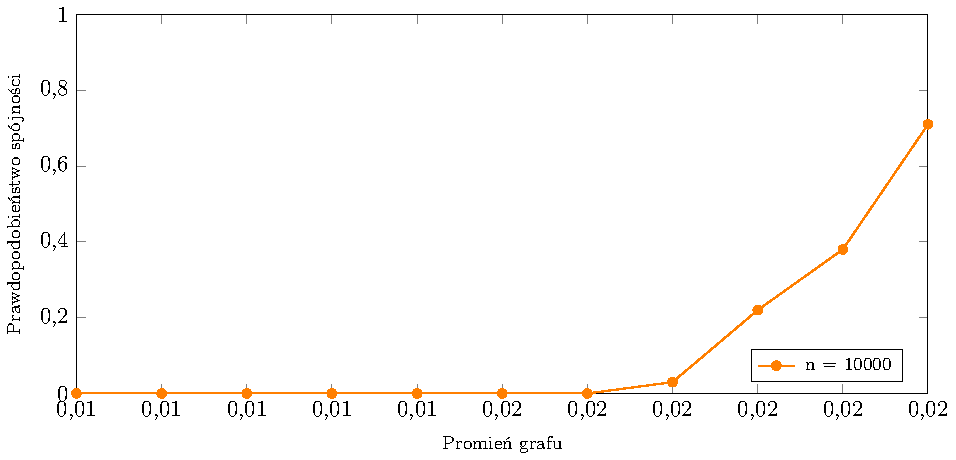
\includepdf[scale=0.9, pages={1}]{10000-0_02_0-consistency_prob.pdf}
		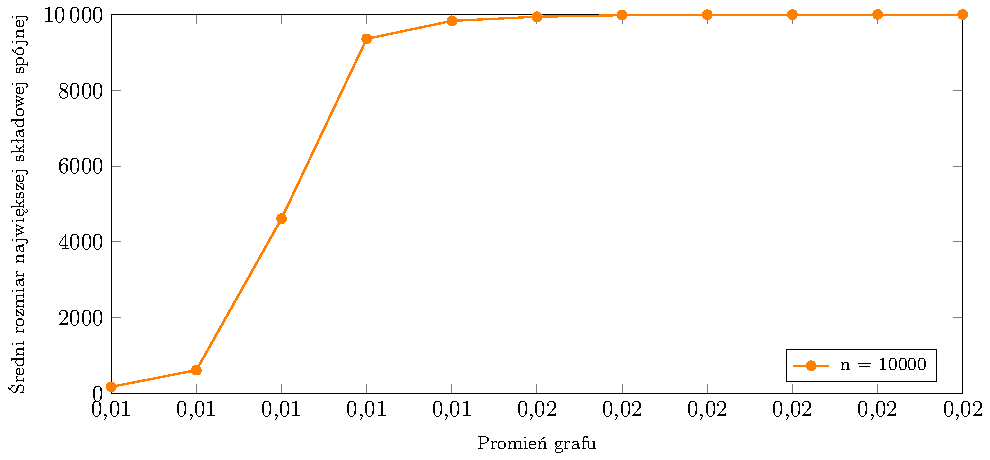
\includepdf[scale=0.9, pages={1}]{10000-0_02_0-max_comps_sizes_means.pdf}
		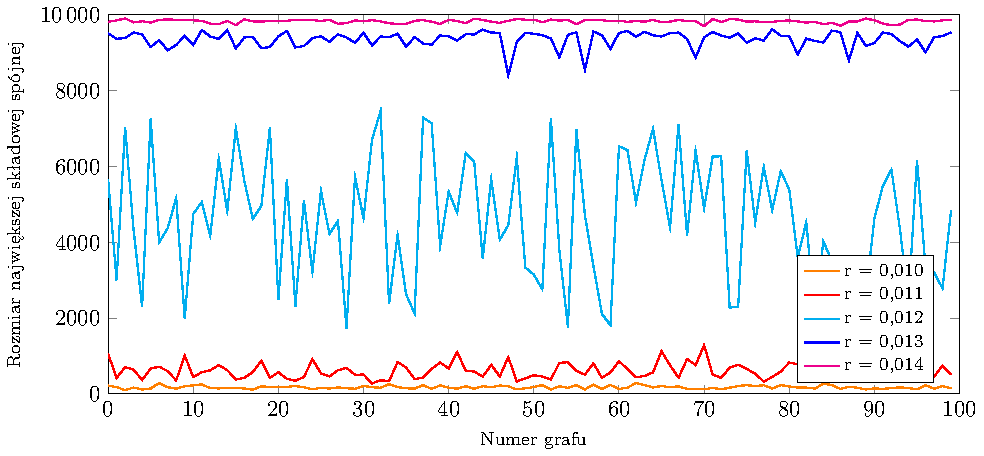
\includepdf[scale=0.9, pages={1}]{10000-max_comps_sizes.pdf}
		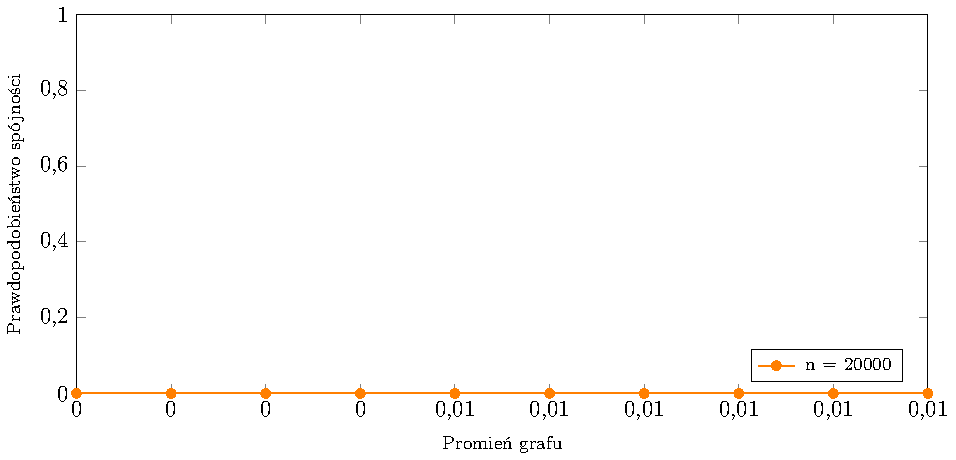
\includepdf[scale=0.9, pages={1}]{20000-0_01_0-consistency_prob.pdf}
		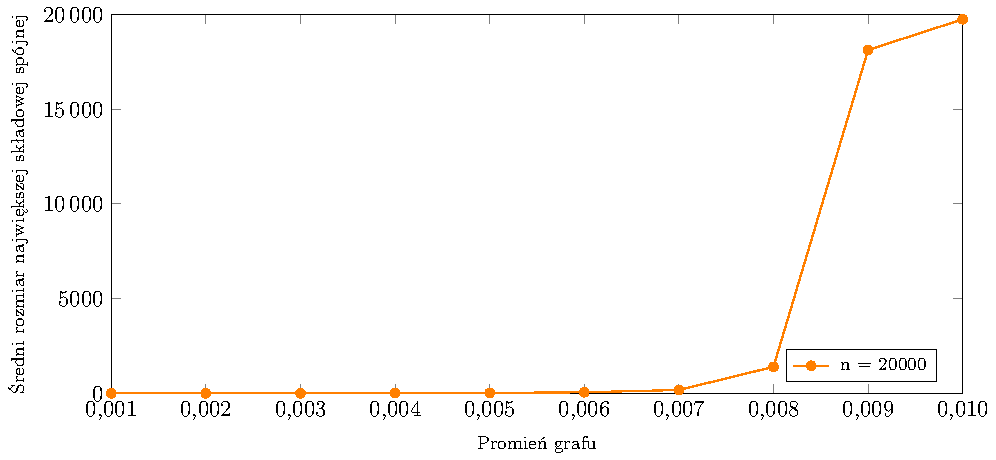
\includepdf[scale=0.9, pages={1}]{20000-0_01_0-max_comps_sizes_means.pdf}
		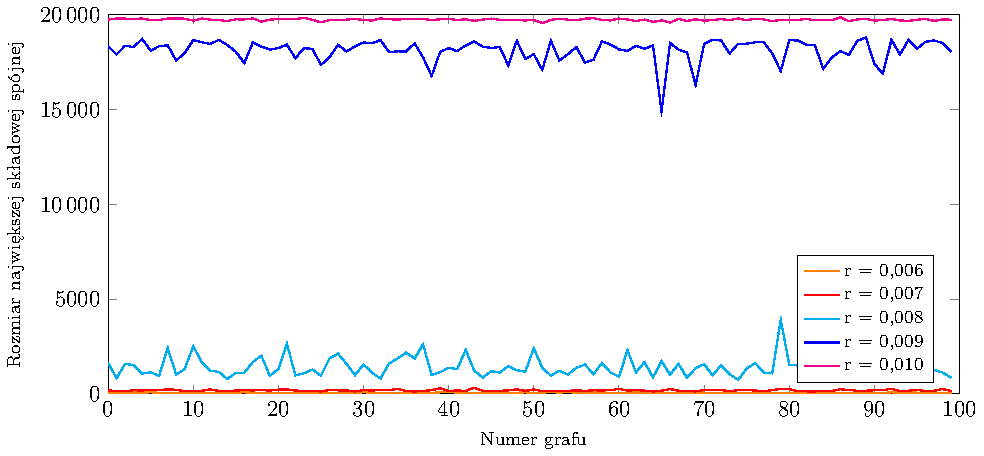
\includepdf[scale=0.9, pages={1}]{20000-max_comps_sizes.pdf}

	\subsection{Wnioski}
		\label{final:testy:wnioski}
	% \\
	% Wnioski na temat prawdopodobiensta spojnosci sieci itp itd.
